\title{KNIME - Konstanz Information Miner}


\author{Harshad Pitkar}
\orcid{1234-5678-9012}
\affiliation{%
  \institution{Indiana University}
  \city{Bloomington} 
  \state{Indiana} 
  \postcode{47408}
}
\email{hpitkar@iu.edu}



% The default list of authors is too long for headers}
\renewcommand{\shortauthors}{Harshad Pitkar}


\begin{abstract}

KNIME also known as Konstanz information miner is an open source
analytics platform that provides a drag and drop GUI interface for
components involved in building a data pipeline such as loading data
from disparate sources, agrregation, data exploration, statistical
functions, machine learning algorithms and finally visualization.
KNIME support reading from a variety of popular formats including csv,
excel, json and xml to name a few. It supports reading data from a
wide range of databases and supports accessing them using jdbc or a
product specific connector for Microsoft SQL server, MySQL and others.
KNIME supports a veriety of machine learning algorithms for
regression, classification, PCA and so on. It also provides deep
learning framework through Keras which enables users to use a variety
of deep learning frameworks such as TensorFlow, cognitive tool
kit~\cite{hid-sp18-517-kdl}. A workflow is a collection of nodes where
a node is a single unit or a step that does processing such as reading
from files, connecting to a database. Nodes are connected to other
nodes in a wprkflow. The GUI interface that provides drag and drop
interface and facilitates the building of a workflow is called a
workbench.

\end{abstract}

\keywords{517, KNIME, Workflow, Text, mining}


\maketitle

\section{Introduction}

The world of information technology is experiencing Data deluge
sometimes also refered as the Data Tsunami wherein almost every
organization is trying to make sense of all the data that is being
collected. Almost every company has invested or is planning invest
into big data projects. Analytics and predictive analytics has been
the key to this process. Naturally, we see an array of tools, open
source to commercial being introduced frequently to support the
analytics requirements. In most cases, the analytics process
progresses through a series of steps from data loading, wrangling,
cleaning to make it ready for performing analysis and building machine
learning models to bring out the value from data.  The entire process
requires multiple tools, programming as well as manual steps.  KNIME
analytics platform works at all these steps and provides an
abstraction layer to all the underlying complexities. KNIME provides a
GUI interface that is user friendly and takes out the complexities of
writing complex code to perform tasks and build models. Subsequent
sections will provide more insight into KNIME tool its features and
how they can be leveraged to complete an analytics project.  The
popularity and success of KNIME is obvious by the fact that Gartner
has placed KNIE as leader in Data Science and Machine learning
platform from 2013 to 2018~\cite{hid-sp18-517-dsml}.

\section{Architecture}
KNIME software is bundled with multiple components such as KNIME
analytics platform which forms the core of the tool, KNIME server that
provides the scalability. KNIME extensions enable the integration with
other open source projects including Apache hadoop. Finally it also
support community and partner extensions which makes it favourable for
all environments~\cite{hid-sp18-517-ksw}.  See
Figure~\ref{fig:knimearch}

\begin{figure}[!ht]
	\centering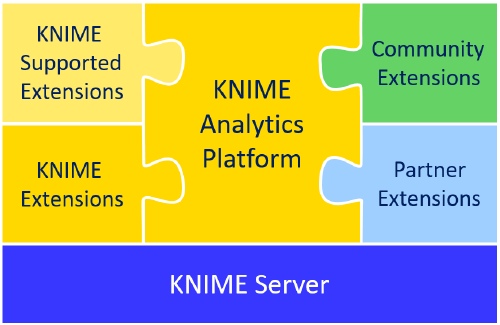
\includegraphics[width=\columnwidth]{../images/knimearch.png}
	\caption{KNIME Architecture~\cite{hid-sp18-517-ksw}}
 	\label{fig:knimearch}
\end{figure}

\subsection{KNIME Analytics platform}
KNIME analytics is the core of the product and is built on eclipse and
hence you would notice the interface is somewhat similar to
eclipse. It's grahical and user friendly interface enables faster data
science cycles and makes it easier to learn as well. It can be
installed on Windows, MAC and linux and comes with many ready to run
examples~\cite{hid-sp18-517-kap}.

A node is a smallest processing unit in KNIME and it supposed to
perform a specific task for example loading of a csv file. Similarly
collection of a nodes sequenced in order makes a workflow. Nodes
within a workflow may be connected to each other and output of one
node could be an input to the other depending on the
sequence~\cite{hid-sp18-517-kintro}.

The GUI interface is divided into multiple sections, mainly workbench,
workflow coach, explorer and the node repository. Workbench is the
area on which you actually drag and drop nodes. For example, if I have
to read a csv file and load it into a database, I would create a node
by dragging the read node type on the workbench followed by a
read-write node of the database type and link them, naturally,
additional configuration of columns and so on would be needed.  An
interesting feature of KNIME is Workflow coach which is an inbuilt
recommender system that provides recommendations on what type of node
to use as the next step, these recommendations are built based on the
community usage of those type of nodes~\cite{hid-sp18-517-ch1sec1}.
KNIME analytics platform includes extensive data visualization
capabilities that allows users to create interactive dashboards,
charts and graphs~\cite{hid-sp18-517-ch5}.

\subsection{KNIME Server}
In a large scale implementation, scalability can be achieved by
deploying a KNIME server. KNIME server scales the platform from an
individual to a group or a team of data scientists and facilitates
collaboration, deployment and management
functionalities~\cite{hid-sp18-517-server}. KNIME server is available
in three editions small, medium and large based on number of users and
features. Small edition is suitable for a smaller teams and has no
support available except for forum access whereas medium and large
offer higher number of users and more features including the ability
to deploy workflows as REST API~\cite{hid-sp18-517-editions}.  KNIME
server allows you to better manage access control at all levels such
as nodes, file and application level. It allows the Data Scientists to
run their workflows on a central server that provides better
performance and handles large datasets. Its web interface allows users
to access the workflows and analytics platform on any device which
also includes REST services~\cite{hid-sp18-517-editions}.

KNIME cloud option makes KNIME Analytics platform and KNIME server
available in cloud through AWS as well as Microsoft
Azure~\cite{hid-sp18-517-cloud}.

\subsection{Extensions}
KNIME supports both open source and commercial extensions that help in
integrating with the analytics platform. This enables the users to
integrate R or python within the workflow. Similarly Apache Hadoop,
Spark and other Big Data open source projects can be integrated with
KNIME through respective estensions. A good Big Data integration
example is being able to import or export data from HDFS or performing
analytics using Hive, Impala that are setup as KNIME nodes in a
workflow~\cite{hid-sp18-517-ksw}. The Big Data connectors are all open
source and are certified by leading hadoop platforms such as cloudera,
hortonworks and mapr~\cite{hid-sp18-517-bde}.  Similarly, extension
for Apache Spark extensions is a set of nodes that enable a variety of
tasks such as data manipulation, machine learning and so
on~\cite{hid-sp18-517-spark}.  For not so savvy developers this serves
as a biggest advantage as they can still complete all the steps
without actually having to write code. Ofcourse there is an option to
write your scripts and use them in the nodes if you wish.


Big data extensions are included in the platform and include those for
Apache Hadoop, Spark that enable reading and writing from HDFS, Hive
as well as Impala. This extension as such provides a graphical
interface for big data applications.

\section{Analytics}
KNIME Analytics: KNIME provides deep learning capability through KNIME
analytics platform that enables users to create, train and execute
deep learning models. Also allows integration with Keras that enables
users to use deep learnign frameworks such as Tensorflow and
others~\cite{hid-sp18-517-dl}. In the meachine learning space it
supports all majority of predictive modeling algorithms for
regression, classigication, Neural networks, Naive Bayes and most of
the tree based models~\cite{hid-sp18-517-pml}.

It also supports transferring data from and to H2O
~\cite{hid-sp18-517-h20} which is a popular open source machine
learning platform~\cite{hid-sp18-517-knimeh20}.

\section{REST support}

If your project involves fetching data through a REST API then KNIME
Workflow allows you to configure nodes that can get data from these
available REST services~\cite{hid-sp18-517-knimeapi}.  KNIME server
also makes it possible to create a service that can be called using
post and get methods.  Again all this can be done using KNIME workflow
and nodes on drag and drop graphical user
interface~\cite{hid-sp18-517-knimerest}.

\section{Simple Workflow}
Lets consider an example of reading a ascii data file cluster the data
and also visualizing the data on a scatter plot. See
Figure~\ref{fig:noderep} Steps included in building such a workflow
are, first we add a node that can read the data file.  Note that
adding node is nothing but dragging the File reader node from the Node
Repository list onto the workbench. The next step is to configure the
node so it know what file to read and the location where it is stored.
The next step would be to add the k-means node which can be found
under the mining section. In the next step we add the last node that
is the color node, this node will assign a unique color to the
different categories in the dataset. See Figure~\ref{fig:kmean}
Finally all the nodes should be connected to each other serially. When
the workflow is executed it reads the data file, applied k-means
algorithm to classify data and the classified data points are plotted
on the scatter plot with a unique color assigned to each
category~\cite{hid-sp18-517-wf}.  Row filtering and columns filtering
nodes are also available that can be used to select only required
columns or filter data based on the values in rows. Both simple and
complex rules can be applied based on the search criteria and can be
achieved using advanced filter~\cite{hid-sp18-517-filters}.  KNIME
also allows aggregating data, bining of data, joining of data as well
as left, right, inner and outer joins~\cite{hid-sp18-517-join}.

\begin{figure}[!ht]
	\centering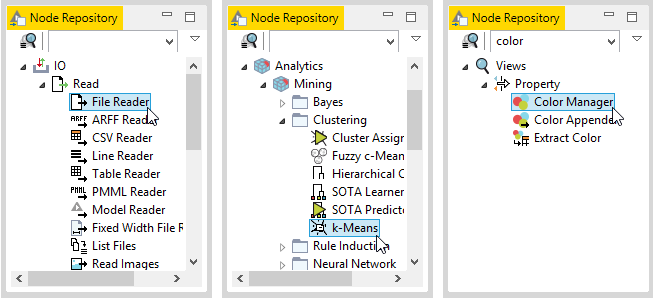
\includegraphics[width=\columnwidth]{../images/node_repositories.png}
	\caption{Node Repositories~\cite{hid-sp18-517-wf}}
 	\label{fig:noderep}
\end{figure}

\begin{figure}[!ht]
	\centering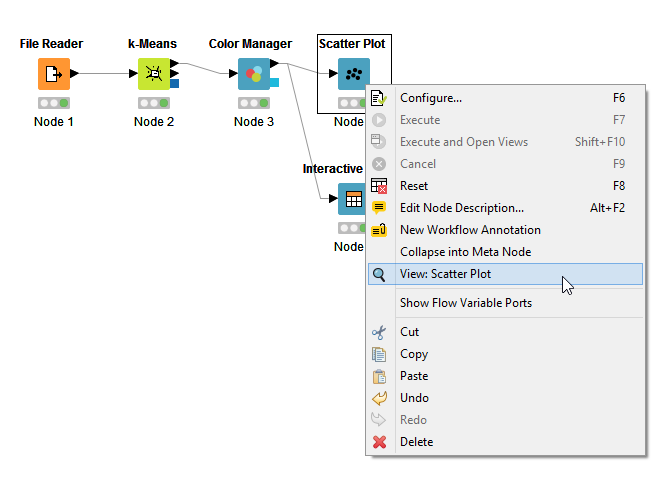
\includegraphics[width=\columnwidth]{../images/kmeans_flow.png}
	\caption{k-means flow~\cite{hid-sp18-517-wf}}
 	\label{fig:kmean}
\end{figure}


\section{Applications}

KNIME is used in almost every domain from government to pharma to
manufacturing, some of common applications of KNIME are Social media
mining, sentiment analysis, credit scoring, energy use prediction,
outlier detection in medical claims, recommender systems, address
deduplication and so on~\cite{hid-sp18-517-applications}.  While KNIME
is Open Source, KNIME AG extends the same analytics platform with
extensions to offer increased productivity and
collaboration~\cite{hid-sp18-517-opensource}.  Ninety percent of the
revenue comes from licenses and most of that is used to add new
features and development~\cite{hid-sp18-517-opensource}.

\section{Conclusion}

In todays world of analytics which is heavily focussed on scripting,
using of analytical tools such as R or python to perform various tasks
in Data science cycle, KNIME provides not only an easy to use
Graphical user interface but supports an array of integrations which
makes it a good choice. It has options for scalability and the user
friendly GUI take out the need to know scripting and every
command. It's easy integration with the popular hadoop platforms,
availability of extensions and above all the user friendly interface
definitely takes out significant amount of complexity from the
analysis process.

\begin{acks}

  The authors would like to thank Dr.~Gregor~von~Laszewski for his
  support and suggestions to write this paper.

\end{acks}

\bibliographystyle{ACM-Reference-Format}
\bibliography{report} 

